\documentclass[10pt,t,english,aspectratio=1610]{beamer}
\usepackage{fontawesome}
\usepackage{graphicx}
\usepackage{array}
\usepackage[normalem]{ulem}
\usepackage{amsfonts,amsmath,amssymb,bm,bbm}
\usepackage{mathrsfs}
% NOTE: sgame is intentionally NOT used -- its `game` environment is
% incompatible with the `array` package (required by colortbl/makecell/multirow)
% and errors with "Missing # inserted in alignment preamble". We use the modern
% TikZ-based `xgames` package instead (loaded after TikZ below).
\usepackage{graphicx,pstricks}
\usepackage{xcolor}
\usepackage{colortbl}
\usepackage{makecell}
\usepackage{tikz,tikzsymbols,gnuplottex}
\usetikzlibrary{decorations.pathreplacing,shapes,positioning,arrows.meta,fit,backgrounds,calc}

% --- xgames: TikZ-based game-theory typesetting (matrixgame, gametree,
% beliefspace, automaton). Not on CTAN; xgames.sty + fikz.sty are vendored at
% the repo root. CC BY-SA 4.0 (xgames) / GPL-3.0 (fikz), (c) Benjamin Bernard.
\usepackage{xgames}

% Custom command for shading rows in a matrixgame
% ---------------------------------------------------------------------------
% \shaderow[<fill options>]{<row>}{<first column>}{<last column>}
% Call this inside the matrixgame, after \payoffmatrix
% Can wrap in a \foreach to shade multiple regions
% Example: \foreach \i in {1,...,5}{ \shaderow[green!50!black]{\i}{\i}{5} }
\newcommand{\shaderow}[4][red!60]{%
  \ifnum#3=1\relax\def\xl{0}\else\pgfmathsetmacro{\xl}{\pmtwi[#3-1]}\fi
  \ifnum#2=1\relax\def\yt{0}\else\pgfmathsetmacro{\yt}{\pmthi[#2-1]}\fi
  \pgfmathsetmacro{\xr}{\pmtwi[#4]}%
  \pgfmathsetmacro{\yb}{\pmthi[#2]}%
  \fill[opacity=0.18, #1] ($(pmt1-tl)+(\xl,-\yt)$) rectangle ($(pmt1-tl)+(\xr,-\yb)$);%
}

\usepackage[english]{babel}
\usepackage[utf8]{inputenc}
\usepackage{appendixnumberbeamer}
\usepackage{datetime2}
\usepackage{booktabs}
\usepackage{setspace}
\usepackage{rotating}
\usepackage{multirow}
\usepackage{listings}

\usepackage{natbib}
\bibliographystyle{unsrtnat}
\renewcommand{\bibfont}{\footnotesize}
\renewcommand{\bibsection}{\vspace{-1em}}

%\usepackage{matlab-prettifier} % For enhanced MATLAB highlighting
\lstset{
    language=matlab,
    % Other options for styling (optional)
    basicstyle=\ttfamily\footnotesize, % Font style
    keywordstyle=\color{blue}, % Keyword color
    commentstyle=\color{green!50!black}, % Comment color
    stringstyle=\color{red!70!black}, % String color
    numbers=left, % Line numbers on the left
    numberstyle=\tiny\color{gray}, % Style for line numbers
    frame=single, % Frame around the listing
    breaklines=true, % Allow line breaking
    captionpos=b, % Caption at the bottom
    tabsize=4 % Tab size
}

% ------------------------------------------------------------------------------
% Use the beautiful metropolis beamer template
% ------------------------------------------------------------------------------
\usepackage[T1]{fontenc}
\usepackage[utf8]{inputenc}
\usepackage{fontawesome}
\usepackage{FiraSans} 
\mode<presentation>
{
  \usetheme[progressbar=foot,background=light]{metropolis} 
  \usecolortheme{default} % or try albatross, beaver, crane, ...
  \usefonttheme{default}  % or try default, serif, structurebold, ...
  \setbeamertemplate{navigation symbols}{}
  \setbeamertemplate{caption}[numbered]
  %\setbeamertemplate{frame footer}{My custom footer}
  \makeatletter
    \setbeamertemplate{frametitle continuation}{}
  \makeatother
} 
\addtobeamertemplate{frametitle continuation}{}{%
  \setbeamertemplate{frametitle continuation}{}%
}
\setbeamertemplate{frametitle continuation}{}

\newenvironment{stepenumerate}{\begin{enumerate}[<+->]}{\end{enumerate}}
\newenvironment{stepitemize}{\begin{itemize}[<+->]}{\end{itemize} }
\newenvironment{stepenumeratewithalert}{\begin{enumerate}[<+-| alert@+>]}{\end{enumerate}}
\newenvironment{stepitemizewithalert}{\begin{itemize}[<+-| alert@+>]}{\end{itemize} }

\newtheorem{question}{Question}
\newtheorem{claim}{Claim}
\newtheorem{proposition}{Proposition}
\newtheorem{remark}{Remark}
\newtheorem{conjecture}{Conjecture}

\definecolor{metrop}{RGB}{29, 44, 44}
\colorlet{GrayLight}{black!15}
\colorlet{GrayMedium}{black!30}
\colorlet{ForestGreen}{green!60!black}

\newenvironment{transitionframe}{
  \setbeamercolor{background canvas}{bg=black!80}
  \begin{frame}}{
    \end{frame}
}

\newcommand{\bsk}{

\bigskip

}

\newcommand{\pd}{\partial}
\newcommand{\RR}{\mathbb{R}}

\newcommand*\hugme[1]{\tikz[baseline=(char.base)]{\node[shape=ellipse,draw,inner sep=0pt] (char) {#1};}}

\newcounter{saveenumi}
\newcommand{\seti}{\setcounter{saveenumi}{\value{enumi}}}
\newcommand{\conti}{\setcounter{enumi}{\value{saveenumi}}}
\resetcounteronoverlays{saveenumi}



\newcommand\dotprod[2]{\langle #1 , #2 \rangle}
\newcommand{\ft}[1]{\widehat #1}
\newcommand{\qabove}[1]{\overset{\text{\large \textbf ?}}{#1}}
\newcommand{\eqae}{\overset{\text{a.e.}}{=}}
\newcommand{\calp}{\mathcal{P}}
\newcommand{\calg}{\mathcal{G}}
\newcommand{\calb}{\mathcal{B}}
\newcommand{\textd}{\text{d}}
\newcommand{\bbr}{\mathbb{R}}
\newcommand{\binm}{\mathbin{M}}
\newcommand{\binc}{\mathbin{C}}
\newcommand{\binb}{\mathbin{B}}
\newcommand{\calc}{\mathcal{C}}
\newcommand{\calh}{\mathcal{H}}
\newcommand{\bfone}{\mathbf{1}}
\newcommand{\bbe}{\mathbb{E}}
\newcommand{\bfle}{\mathbf{e}}
\newcommand{\calf}{\mathcal{F}}
\newcommand{\cala}{\mathcal{A}}
\newcommand{\cale}{\mathcal{E}}
\newcommand{\bbn}{\mathbb{N}}
\newcommand{\cantor}{\calc}
\newcommand{\calY}{\mathcal{Y}}
\newcommand{\textb}{\text{B}}
\newcommand{\calm}{\mathcal{M}}
\newcommand{\bint}{\mathbin{T}}
\newcommand{\ep}{\epsilon}
\newcommand{\bbq}{\mathbb{Q}}
\newcommand{\bbp}{\mathbb{P}}
\newcommand{\cals}{\mathcal{S}}
\newcommand{\emptysequence}{e}
\newcommand{\bbz}{\mathbb{Z}}
\newcommand{\fraka}{\frak{A}}
\newcommand{\frakb}{\frak{B}}
\newcommand{\length}{\text{length}}
\newcommand{\bfn}{\mathbf{N}}
\newcommand{\support}{\text{support}}
\DeclareMathOperator*{\argmax}{arg\,max}
\newcommand{\dom}{\mbox{dom}}
\def\ut{\underline t}
\def\um{\underline m}
\def\PP{\mathbb{P}}
\def\EE{\mathbb{E}}
\def\RR{\mathbb{R}}

% Title page info
\title[Repeated Games]{Repeated Games (Not in the Book)}
\author[ECON 5001]{ECON 5001\\Prof. Paul J. Healy} \color{metrop}
\institute[OSU]{}
\date[]{\vfill {\tiny Updated \today\ at\ \DTMcurrenttime}}

% ---------------------------------------------------------------------
% SCOPE AND NOTATION
%   Not in Bonanno. Complete information, perfect monitoring, pure
%   strategies only. Uses only SPNE / backward induction (Ch 3-4, 7).
%   a^t = action profile in period t. h_t = (a^1,...,a^{t-1}), h_1 = empty.
%   s_i(h_t) = Player i's action after history h_t.
%   Two-period game: payoffs are summed (no discounting).
%   Infinite game: U_i = sum_t delta^{t-1} u_i(a^t). Folk theorem stated
%   in per-period average terms, (1-delta) U_i.
%
% ANSWERS (all checked numerically)
%   Stage game G (two-period example): rows T,M,B; cols L,C,R
%       L    C    R
%   T  1,1  5,0  0,0
%   M  0,5  4,4  0,0
%   B  0,0  0,0  3,3
%     Pure stage NE: (T,L) = (1,1) and (B,R) = (3,3). (M,C) is not a NE
%     (T beats M vs C: 5 > 4).
%     Punishment strategy: period 1 play M (P1) / C (P2). Period 2:
%     (B,R) if period 1 was (M,C), else (T,L).
%       Conform: 4 + 3 = 7. Best deviation (T): 5 + 1 = 6. So SPNE.
%     Period-2 histories: 9. A strategy = 1 + 9 = 10 choices.
%     Pure strategies per player: 3^10 = 59,049.
%   PD, Cooperate/Defect: (2,2) (0,3) (3,0) (1,1). Read as deck 03's
%   food-truck price war: Cooperate = Normal price, Defect = cut prices
%   (deck 03's "Discount"; slides avoid that word next to delta).
%     Two periods: period 2 is (D,D) after every history, so period 1
%     is (D,D) too. Any finite T: Defect always (unique SPNE).
%     Grim trigger: 2/(1-d) >= 3 + d/(1-d)  <=>  d >= 1/2.
%     At d = .9: conform 20, deviate 3 + 9 = 12.
%     r = 10%: $90.91 today = $100 next year; d = 1/1.1 = .909.
%     $100 in two years is worth $82.64 today.
%     Always Cooperate vs Always Cooperate is NOT an SPNE (defect forever
%     against an unconditional cooperator: 3/(1-d) > 2/(1-d)).
%     Minmax = 1 for each player.
%   MobLab: PD (Matrix). Game 1 = exactly 4 rounds. Game 2 = Minimum
%     Rounds 1, Ending Probability 25% (continue .75, expected length 4).
%     MobLab says its default payoffs support grim trigger iff ending
%     probability <= 50%, i.e. d >= 1/2, same threshold as our PD.
%   Worked example (Shell vs Speedway, prices High/Low):
%            H      L
%     H   6,4    1,6
%     L   8,1    3,2
%     Both have L dominant; stage NE (L,L) = (3,2).
%     Minmax: Shell 3, Speedway 2 (pure; mixing doesn't lower them).
%     Grim: Shell 6 >= 8(1-d) + 3d -> d >= 2/5. Speedway 4 >= 6(1-d)+2d
%       -> d >= 1/2. Grim is an SPNE iff d >= 1/2 (Speedway binds).
%       d = 1/2 <-> r = 100%.
%     Cut noticed one period late: Shell 6 >= 8(1-d^2) + 3d^2 ->
%       d^2 >= 2/5, d >= .632. Speedway 4 >= 6(1-d^2) + 2d^2 ->
%       d^2 >= 1/2, d >= .707.
%     (4,3): feasible (at y=3 the feasible x-range is [2.5, 6.67]) and
%       above minmax (3,2), so folk theorem: yes for d near 1.
%     (2,5): feasible (x-range at y=5 is [1.5, 3.5]) but Shell 2 < 3: no.
%   Practice: (C,C) = (2.5,2.5): 2.5 >= 3(1-d) + d  ->  d >= 1/4.
% ---------------------------------------------------------------------

% The two-period stage game, drawn several times
\newcommand{\stagegame}[1][]{%
\begin{matrixgame}[top={L, C, R}, left={T, M, B}, player names={Player 1, Player 2}, #1]
  \payoffmatrix{1,1 & 5,0 & 0,0 \\ 0,5 & 4,4 & 0,0 \\ 0,0 & 0,0 & 3,3}
\end{matrixgame}}

% The PD (deck 03's food-truck price war: Cooperate = Normal price,
% Defect = cut prices)
\newcommand{\pdgame}[1][]{%
\begin{matrixgame}[top={Cooperate, Defect}, left={Cooperate, Defect}, #1]
  \payoffmatrix{2,2 & 0,3 \\ 3,0 & 1,1}
\end{matrixgame}}

\begin{document}

\frame{\maketitle}

\begin{frame}{Where We Left Off}
Prisoners' Dilemma:
\bsk
\centering
\pdgame
\bsk
\raggedright
\textbf{Think of it as a price war}: Dos Hermanos vs.\ Pitabilities
\begin{itemize}
    \item Cooperate $=$ keep prices Normal. Defect $=$ cut prices
    \item \textbf{Interacting every day}: a repeated game!
\end{itemize}
\bsk
\begin{itemize}
    \item Play once: D is strictly dominant
    \item Play repeatedly: Can we enforce Cooperation?
\end{itemize}
\vspace{-0.3in}
\end{frame}

% ==============================================================
% MOBLAB --- PLAY FIRST
% ==============================================================

% ---- MobLab run: Prisoner's Dilemma (Matrix) ------------------------
% Two games in one playlist, same partner within a game, new partner
% between games:
%   Game 1: exactly 4 rounds (students are told it's 4).
%   Game 2: Minimum Rounds = 1, Ending Probability = 25%
%           (75% chance of another round; expected length 4).
% MobLab's guide: with default payoffs, grim trigger supports
% cooperation iff the ending probability is <= 50%. If the config lets
% you enter payoffs, 8,8 / 0,12 / 12,0 / 4,4 (our PD x 4) keeps
% the deck's numbers. Results come back in "Back to MobLab".
% ---------------------------------------------------------------------
\begin{frame}{MobLab: ``Prisoner's Dilemma (Matrix)''}
\begin{itemize}
    \item MobLab time!
    \item Twice-repeated PD game
    \item Play the PD game twice with the same partner
    \item Repeat with a new partner
    \begin{itemize}
        \item They can't see how you played previously
    \end{itemize}
\end{itemize}
\vfill
\centering
Feel free to talk! And play it the way you'd actually play it.
\vspace{-0.2in}
\end{frame}

% ==============================================================
% TWO PERIODS
% ==============================================================

\begin{frame}[standout]
Playing Twice Can Introduce New Nash Equilibria
\end{frame}

\begin{frame}{Example}
\begin{columns}[T]
\begin{column}{0.5\textwidth}
\centering
\only<1>{\stagegame}%
\only<2->{\stagegame[br]}
\end{column}
\begin{column}{0.48\textwidth}
Pure NE: \underline{\hspace{1.2in}}
\bsk
``Best'' Outcome: \underline{\hspace{0.8in}}
\bsk
\onslide<3->{Is $(M,C)$ a NE? \underline{\hspace{0.6in}}}
\end{column}
\end{columns}
\bsk
\onslide<4->{Now play it \textbf{twice}:
\begin{itemize}
    \item Period 1: play the game. Everyone sees what happened
    \item Period 2: play it again
    \item Total payoff $=$ period 1 payoff $+$ period 2 payoff
\end{itemize}}
\bsk
\onslide<5->{Can $(M,C)$ happen in period 1???}
\vspace{-0.3in}
\end{frame}

\begin{frame}{A Strategy With a Threat}
\begin{columns}[T]
\begin{column}{0.5\textwidth}
\centering
\stagegame
\end{column}
\begin{column}{0.48\textwidth}
\textbf{Period 1:} Play $(M,C)$
\bsk
\textbf{Period 2:}
\begin{itemize}
    \item If $(M,C)$ happened: play $(B,R)$
    \item Otherwise: play $(T,L)$
\end{itemize}
\end{column}
\end{columns}
\bsk
Reward with the good NE. Punish with the bad NE
\bsk
Check P1 in period 1:
\begin{itemize}
    \item Conform ($M$): \ \underline{\hspace{0.3in}} $+$ \underline{\hspace{0.3in}} $=$ \underline{\hspace{0.3in}}
    \item Deviate ($T$): \ \underline{\hspace{0.3in}} $+$ \underline{\hspace{0.3in}} $=$ \underline{\hspace{0.3in}}
\end{itemize}
\bsk
\onslide<2->{Period 2? \ Playing a NE either way, no incentive to deviate}
\vspace{-0.3in}
\end{frame}

\begin{frame}{Every Period-2 Subgame}
After period 1, there are \underline{\hspace{0.3in}} possible \textbf{histories}.
\bsk
\textbf{History:} What's happened so far in the game ($(T,L)$, $(T,C)$, $(M,B)$, etc.)
\bsk
Period 2: Strategies can respond to the history
\bsk
After history $(M,C)$: play $(B,R)$\\
After any other history: play $(T,L)$
\bsk
SPNE: Solve via backward induction.
\bsk
\onslide<2->{\textbf{Lesson:} Period 2 can be used to \textbf{punish} \& \textbf{reward} period 1 behavior\\}
\onslide<3->{\textbf{BUT}... what happens in Period 2 better be a NE. Otherwise, not credible}
\vspace{-0.3in}
\end{frame}

% ==============================================================
% FORMALISM
% ==============================================================

\begin{frame}[standout]
Formalizing Repeated Games
\end{frame}

\begin{frame}{Stage Game vs.\ Supergame}
\begin{itemize}
    \item \textbf{Stage game} $G$: the game played each period
    \begin{itemize}
        \item Our $3\times 3$ game, or the PD
    \end{itemize}
    \item \textbf{Supergame} $G^T$: play $G$ in periods $t=1,2,\dots,T$
    \begin{itemize}
        \item Everyone sees all past play
        \item $T$ can be finite or $\infty$
    \end{itemize}
\end{itemize}
\bsk
\begin{columns}[T]
\begin{column}{0.48\textwidth}
\textbf{Action:} what you do in \textbf{one} period
\begin{itemize}
    \item $a_i^t\in A_i$ (eg, $M$)
    \item Profile: $a^t=(a_1^t,a_2^t)$
\end{itemize}
\end{column}
\begin{column}{0.5\textwidth}
\textbf{Strategy:} a complete plan for $G^T$
\begin{itemize}
    \item What to do in \textbf{every} period
    \item ...after \textbf{everything} that could happen
\end{itemize}
\end{column}
\end{columns}
\vspace{-0.3in}
\end{frame}

\begin{frame}{Histories}
\textbf{History} at the start of period $t$: everything that happened before $t$
$$h_t=(a^1,a^2,\dots,a^{t-1})$$
\vspace{-0.15in}
\begin{itemize}
    \item $h_1=\emptyset$ \ (nothing has happened yet)
    \item $H_t=$ set of all possible histories at the start of period $t$
\end{itemize}
\bsk
\textbf{Ex:} Suppose the $3\times 3$ game is played 4 times:
\begin{itemize}
    \item $h_2=(M,C)$ is one history at start of period 2
    \item $h_3=((M,C),(T,L))$ is a possible history at start of period 3
    \item $h_4=((M,C),(T,L),(M,C))$ is a possible period-4 history
    \item $|H_2|=$ \underline{\hspace{0.4in}} \qquad $|H_3|=$ \underline{\hspace{0.8in}} \qquad $|H_4|=$ \underline{\hspace{1in}}
\end{itemize}
\bsk
\onslide<2->{Each history starts a \textbf{subgame} (it's a singleton node in the tree)}
\vspace{-0.3in}
\end{frame}

\begin{frame}{Pure Strategy in a Repeated Game}
\begin{block}{Definition}
A \textbf{pure strategy} for Player $i$ is a function $s_i$ that maps every history to an action: \ $s_i(h_t)\in A_i$ for every $h_t$ in every $H_t$
\end{block}
\bsk
Back to our 2-period $3\times 3$ game. Our threat strategy for P1:
\begin{align*}
s_1(\emptyset)&=\underline{\hspace{0.5in}}\\
s_1\big((M,C)\big)&=\underline{\hspace{0.5in}} \quad \text{when } h_2=(M,C)\\
s_1(h_2)&=\underline{\hspace{0.5in}} \quad \text{for every other } h_2\neq (M,C)
\end{align*}
\bsk
\onslide<2->{P1 moves after how many different histories? \ $1+\underline{\hspace{0.3in}}=\underline{\hspace{0.3in}}$ \\
\# of pure strategies: \ }
\onslide<3->{$3^{10}=59,049$
\bsk
}
\onslide<4->{Imagine chess...}
\vspace{-0.3in}
\end{frame}

\begin{frame}{Two Kinds of Equilibrium}
\textbf{Stage-game NE:} a NE of $G$ (one period)
\begin{itemize}
    \item $(T,L)$ and $(B,R)$ in our example
\end{itemize}
\bsk
\textbf{Equilibrium of the supergame:} a NE or SPNE of $G^T$
\begin{itemize}
    \item A profile of \textbf{strategies} $(s_1,s_2)$, not actions
    \item SPNE: a NE in the subgame after \textbf{every} history
\end{itemize}
\bsk
\textbf{Ex:} our threat strategies are a SPNE of $G^2$
\begin{itemize}
    \item Period-1 play of $(M,C)$ is part of a SPNE
    \item Even though $(M,C)$ is \textbf{not} a stage-game NE!
\end{itemize}
\vfill
\vspace{-0.3in}
\end{frame}

\begin{frame}{Stage NE Every Period Is Always Safe}
Suppose $a^*=(a_1^*,\ldots,a_n^*)$ is a NE of the stage game $G$.
\bsk
Consider the strategy: $s_i(h_t)=a_i^*$ regardless of $h_t$\\
``Always play $a_i^*$, \textbf{regardless} of what happened in the past.''
\bsk
\begin{block}{Theorem}
If $a^*=(a_1^*,\ldots,a_n^*)$ is a NE of the stage game $G$, then all players playing the strategy ``$s_i(h_t)=a_i^*$ for every $h_t$'' is a SPNE of $G^T$.
\end{block}
{\footnotesize Same for any \textbf{sequence} of stage NE that ignores history: $a^{1*}, a^{2*}, \dots$}
\bsk
Why?
\begin{itemize}
    \item Deviating today can't improve today's payoff (b/c it's a NE)
    \item Deviating today can't change tomorrow's payoff (b/c they'll still play $a^*$)
    \item Thus, deviating never improves payoffs
\end{itemize}
\bsk
\textbf{Corollary:} Stage game $G$ is a finite game $\Rightarrow$ $G$ has a NE $\Rightarrow$ There exists an SPNE of $G^T$
\vfill
\vspace{-0.3in}
\end{frame}

% ==============================================================
% FINITE PD
% ==============================================================

\begin{frame}[standout]
Twice-Repeated Prisoners' Dilemma
\end{frame}

\begin{frame}{Two-Period PD}
\begin{columns}[T]
\begin{column}{0.48\textwidth}
\centering
\pdgame
\end{column}
\begin{column}{0.5\textwidth}
Price war over two days\\[6pt]
Try a punishment strategy:
\begin{itemize}
    \item Period 1: $(C,C)$
    \item Period 2: reward if both Cooperated, punish otherwise
\end{itemize}
\bsk
\onslide<2->{\textbf{Problem:} Period 2 plan isn't stage game NE}
\end{column}
\end{columns}
\bsk
\onslide<3->{\textbf{Problem:} only \textbf{one} stage-game NE: $(D,D)$. No credible punishment/reward.}
\vspace{-0.3in}
\end{frame}

\begin{frame}{Any Finite Number of Periods}
\begin{itemize}
    \item Period $T$: last period. Play \underline{\hspace{0.9in}}
    \item Period $T-1$: can't affect period $T$ play. Play \underline{\hspace{0.9in}}
    \item Period $T-2$: ...
    \item ...
    \item Period 1: \underline{\hspace{0.9in}}
\end{itemize}
\bsk
\onslide<2->{\begin{block}{Theorem}
If $G$ has a unique NE and $T$ is finite, the only SPNE of $G^T$ is to play that NE every period.
\end{block}}
\bsk
\onslide<3->{The game \textbf{unravels} from the end.}
\vspace{-0.3in}
\end{frame}

\begin{frame}{But In the Lab...}
\textbf{Lab result:} people \textbf{do} cooperate in finitely repeated PDs
\begin{itemize}
    \item Lots of cooperation early
    \item Collapses in the last few rounds (``end-game effect'')
    \item With experience, the collapse starts earlier
\end{itemize}
\bsk
\textbf{More cooperation} when players aren't sure the other is purely selfish
\begin{itemize}
    \item A little doubt about the other's \textbf{type}...
    \item We'll see this in Chapter 15!
\end{itemize}
\vfill
{\footnotesize Source: Caplan, \textit{A Practicum in Behavioral Economics}, \S3, p.~176.\\ Selten \& Stoecker (1986, \textit{JEBO}); Andreoni \& Miller (1993, \textit{EJ}).}
\vspace{-0.2in}
\end{frame}

% ==============================================================
% INFINITE HORIZON
% ==============================================================

\begin{frame}[standout]
Infinitely Repeated Games: $T=\infty$
\end{frame}

\begin{frame}{No Last Period}
What if the game doesn't have a known end date? So, $T=\infty$
\begin{itemize}
    \item Another interpretation: the game ends at a random time
\end{itemize}
\bsk
\textbf{Problem 1:} Can't apply backward induction/SPNE
\bsk
\onslide<2->{\textbf{Problem 2:} payoffs add up to infinity
\begin{itemize}
    \item Always Cooperate: \ $2+2+2+\cdots=\infty$
    \item Defect once, then get Defected on forever: \ $3+1+1+\cdots=\infty$
\end{itemize}
Which would you prefer?\\
Can't compare $\infty$ to $\infty$}
\bsk
\onslide<3->{\textbf{Fix:} future payoffs count \textbf{less} than today's}
\vspace{-0.3in}
\end{frame}

\begin{frame}{Discounting: Money Now vs.\ Later}
Interest rate $r=10\%$ (for example):
\begin{itemize}
    \item At 10\% interest, \$90.91 today grows to $\$90.91\times 1.10=\$100$ next year
    \item So \$100 next year is worth \underline{\hspace{0.6in}} today
    \item \$82.64 today grows to $\$82.64\times 1.10=\$90.91$ next year, then to \$100 in 2 years
    \item So \$100 in two years is worth \underline{\hspace{0.6in}} today
\end{itemize}
\bsk
General: What amount $x$ today will grow to \$100 in $t$ periods?
\begin{align*}
    x\,(1+r)^t &= 100\\
    x &= \big(\frac{1}{1+r}\big)^t 100 \\
    x &= \delta^t 100
\end{align*}
\textbf{Discount factor} $\bm{\delta}$: how much we discount future payoffs per period: $\delta = 1/(1+r)$\\
\onslide<2->{Skip the $r$ and just work with $\delta$.\\}
\onslide<3->{\textbf{Patient:} don't discount much. $\delta$ near 1\\}
\onslide<4->{\textbf{Impatient:} discount a lot. $\delta$ near 0}
\end{frame}

\begin{frame}{Utility of a Stream of Payoffs}
``Stream'' of payoffs: $u_i^1$ today, $u_i^2$ next period, $u_i^3$ after that, \textit{etc.}
\bsk
\textbf{``Exponential'' discounting:} add them up, discounting each period by another $\delta$.\\
Total value of the stream of payoffs:
$$U_i=u_i^1+\delta u_i^2+\delta^2 u_i^3+\cdots=\sum_{t=1}^{\infty}\delta^{t-1}\,u_i^t$$
\bsk
\onslide<2->{\textbf{Fact:} if $0\le\delta<1$, this is \textbf{finite}}
\bsk
\onslide<3->{\textbf{Important Example:} Suppose the stream pays $x$ every period forever:
$$U_i=x+\delta x+\delta^2x+\delta^3x+\cdots \qquad \delta U_i=\underline{\hspace{1.2in}}$$
$$U_i-\delta U_i=(1-\delta)U_i=\underline{\hspace{0.3in}} \quad\Rightarrow\quad U_i=\underline{\hspace{0.6in}}$$}
\vspace{-0.3in}
\end{frame}

\begin{frame}{The Infinitely Repeated PD}
\begin{columns}[T]
\begin{column}{0.48\textwidth}
\centering
\pdgame
\end{column}
\begin{column}{0.5\textwidth}
One SPNE we already know:
\begin{itemize}
    \item Always Defect, no matter what
    \item Why? \underline{\hspace{1.2in}}
\end{itemize}
\end{column}
\end{columns}
\bsk
\onslide<2->{Powerful strategy: \textbf{Grim Trigger:}
\begin{itemize}
    \item Period 1: play Cooperate
    \item Keep Cooperating as long as \textbf{everyone} always has
    \item Once anyone Defects: you Defect \textbf{forever}
    \item Price war: High prices until someone undercuts. Then low prices forever
\end{itemize}}
\bsk
\onslide<3->{
\begin{tabular}{ccc}
Period $t=1$ & \hspace{1in} & Periods $t>1$ \\
\cline{1-1} \cline{3-3}
$s_i(\emptyset)=C$ & & $s_i(h_t) = \begin{cases}
    C & \text{if} \ \ h_t=(\underbrace{(C,C),(C,C),\ldots,(C,C)}_{t-1\  \text{periods}}) \\
    D & \text{for any other} \ h_t 
\end{cases}$
\end{tabular}
}
\vspace{-0.3in}
\end{frame}

\begin{frame}{Is Grim Trigger a SPNE?}
For SPNE, need to check that there's no profitable deviation in \textbf{any} subgame (history)
\bsk
\textbf{1. Someone already Defected} ($h_t\neq ((C,C),(C,C),\ldots,(C,C))$)
\begin{itemize}
    \item Both Defect forever: $(D,D)$ is the stage game NE every period
    \item Theorem $\Rightarrow$ no profitable deviation \checkmark
\end{itemize}
\bsk
\textbf{2. Everyone always Cooperated} ($h_t= ((C,C),(C,C),\ldots,(C,C))$)
\begin{itemize}
    \item Conform: \ $2+2\delta+2\delta^2+\cdots=$ \underline{\hspace{0.8in}}
    \item Deviate (Defect today, triggering the Grim Trigger response tomorrow):
    \begin{itemize}
        \item Today: \underline{\hspace{0.3in}}
        \item Then punished forever starting tomorrow: \ $\delta1+\delta^21+\delta^31+\cdots$
        \item Total payoff from this plan:\\
        $3+\delta1+\delta^21+\delta^31+\cdots$\\
        $2+\big(1+\delta1+\delta^21+\delta^31+\cdots\big)$\\
        $2+\frac{1}{1-\delta}1$
    \end{itemize}
\end{itemize}
\vspace{-0.2in}
\end{frame}

\begin{frame}{The Threshold}
\textbf{In words:} cooperating forever must beat grabbing 3 today and getting punished forever\\
{\footnotesize Price war: is one day of extra sales from a price cut worth a price war forever?}
\bsk
$$\underbrace{2\frac{1}{1-\delta}}_{\text{cooperate forever}}\ \ \ge\ \ \underbrace{2+\frac{1}{1-\delta}1}_{\text{grab today, punished forever}}$$
\bsk
Solve for $\delta$:
\onslide<2->{
\begin{align*}
    2 &\geq 2(1-\delta) + 1\\
    1 &\geq 2(1-\delta)\\
    1 &\geq 2-2\delta\\
    2\delta &\geq 1\\
    \delta &\geq 1/2
\end{align*}
}
\onslide<3->{\textbf{Result:} Grim Trigger is a SPNE $\iff \delta\ge$ \underline{\hspace{0.4in}}. In other words, if they're \uline{patient enough}}
\end{frame}

% \begin{frame}{Back to MobLab}
% \vspace{0.1in}
% \centering
% \renewcommand{\arraystretch}{2}
% \begin{tabular}{l|c|c|c|c|c|}
% \cline{2-6}
%  & Round 1 & Round 2 & Round 3 & Round 4 & Round 5+ \\
% \hline
% \multicolumn{1}{|l|}{Game 1: \% cooperate} & \hspace{0.45in} & \hspace{0.45in} & \hspace{0.45in} & \hspace{0.45in} & --- \\
% \hline
% \multicolumn{1}{|l|}{Game 2: \% cooperate} & & & & & \\
% \hline
% \end{tabular}
% \bsk
% \raggedright
% Game 2: $\delta=$ \underline{\hspace{0.5in}}. MobLab's payoffs: Grim Trigger works iff $\delta\ge\tfrac12$
% \vfill
% {\footnotesize Lab result: cooperation rises with $\delta$. Dal B\'o (2005, \textit{AER}); Dal B\'o \& Fr\'echette (2011, \textit{AER}).}
% \vspace{-0.2in}
% \end{frame}

\begin{frame}{Other Strategies}
\begin{itemize}
    \item \textbf{Tit-for-Tat:} start with Cooperate, then copy what they did last period
    \begin{itemize}
        \item Won Axelrod's computer tournaments (1980)
        \item Nice, retaliatory, forgiving
    \end{itemize}
    \item \textbf{Always Cooperate}, no matter what
    \begin{itemize}
        \item Is playing ``Cooperate at every history'' a SPNE? \underline{\hspace{0.8in}}
    \end{itemize}
    \item \textbf{Always Defect}: always a SPNE
\end{itemize}
\bsk
\onslide<2->{\textbf{Lesson:} cooperation needs a credible \textbf{threat}}
\vfill
{\footnotesize Not in the book. Axelrod, \textit{The Evolution of Cooperation} (1984). Tit-for-Tat was submitted by Anatol Rapoport.}
\vspace{-0.2in}
\end{frame}

\begin{frame}{This Is Everywhere}
Repeated PDs, with cooperate / defect in each:
\begin{itemize}
    \item \textbf{Cartels:} OPEC members: stick to quota / pump more
    \item \textbf{Price wars:} airlines on a route: hold fares / slash fares
    \item \textbf{Trade:} countries: keep tariffs low / raise tariffs
    \item \textbf{Roommates:} do your chores / let them pile up
    \item \textbf{Online sellers:} ship what you promised / ship junk
    \item \textbf{WWI trenches:} live and let live / non-stop combat
\end{itemize}
\bsk
In each: the \textbf{future} keeps people honest today
\vfill
{\footnotesize Trenches: ``live and let live,'' Axelrod (1984). Many historians disagree.}
\vspace{-0.2in}
\end{frame}

\begin{frame}{But Those Are More Complicated}
Real versions add:
\begin{itemize}
    \item \textbf{Imperfect monitoring:} you can't directly see what your opponent did
    \begin{itemize}
        \item e.g., you don't see their price cut, but you see a drop in your demand
    \end{itemize}
    \item \textbf{Many players:} whom do you punish?
    \item \textbf{Entry:} new players who weren't part of the original agreement
    \item \textbf{Renegotiation:} after a price war, both want to ``let bygones be bygones''
\end{itemize}
\bsk
Core tension survives: today's gain vs.\ tomorrow's punishment.\\
And, is tomorrow's punishment even credible?
\vspace{-0.3in}
\end{frame}

% ==============================================================
% FOLK THEOREM
% ==============================================================

\begin{frame}[standout]
How Much Can Repetition Do?
\end{frame}

\begin{frame}{Minmax Payoff in the PD}
\centering
\begin{matrixgame}[top={Cooperate, Defect}, left={Cooperate, Defect}]
  \payoffmatrix{2,2 & 0,3 \\ 3,0 & 1,1}
\end{matrixgame}
\raggedright
\begin{itemize}
    \item You're the row player
    \item Suppose your opponent wants to punish you for your past behavior
    \item<2-> How much can they hurt you?
    \item<3-> Can they force you to zero payoff?
    \begin{itemize}
        \item They play $D$ and you play $C$
    \end{itemize}
    \item<4-> No! You'd switch to $D$ and get 1, not zero
\end{itemize}
\bsk
\onslide<5->{\textbf{Minmax Payoff:} the lowest payoff that others can force you to accept}
\bsk
\onslide<6->{In this game: Your minmax payoff is 1}
\end{frame}

\begin{frame}{Minmax Payoff}
\textbf{In words:} the worst the others can hold you to, if you always best respond
$$v_i=\underbrace{\min_{a_{-i}}}_{\text{others hurt you}}\ \ \underbrace{\max_{a_i}\ u_i(a_i,a_{-i})}_{\text{you best respond}}$$
\bsk
\textbf{Ex:} in the previous slide, $v_i=1$ for both players
\bsk
\onslide<2->{\textbf{Fact:} You can always get at least $v_i$. Thus, no SPNE can give you less than $v_i$}
\end{frame}

\begin{frame}{Feasible Payoffs}
\begin{columns}[c]
\begin{column}{0.52\textwidth}
\centering
\begin{tikzpicture}[scale=1.15]
  \draw[->] (0,0) -- (3.6,0) node[right] {$u_1$};
  \draw[->] (0,0) -- (0,3.6) node[above] {$u_2$};
  \foreach \x in {1,2,3} {\draw (\x,0.06) -- (\x,-0.06) node[below] {\small \x};}
  \foreach \y in {1,2,3} {\draw (0.06,\y) -- (-0.06,\y) node[left] {\small \y};}
  \only<2->{\fill[blue!12] (0,3) -- (2,2) -- (3,0) -- (1,1) -- cycle;
            \draw[blue!60, thick] (0,3) -- (2,2) -- (3,0) -- (1,1) -- cycle;}
  \only<3->{\fill[red!25] (1,1) -- (1,2.5) -- (2,2) -- (2.5,1) -- cycle;
            \draw[red!70, dashed] (1,0) -- (1,3.3);
            \draw[red!70, dashed] (0,1) -- (3.3,1);}
  \fill (2,2) circle (1.6pt) node[above right, font=\scriptsize] {(C,C)};
  \fill (0,3) circle (1.6pt) node[right=2pt, font=\scriptsize] {(C,D)};
  \fill (3,0) circle (1.6pt) node[above right, font=\scriptsize] {(D,C)};
  \fill (1,1) circle (1.6pt) node[below left, font=\scriptsize] {(D,D)};
\end{tikzpicture}
\end{column}
\begin{column}{0.46\textwidth}
Per-period average payoffs
\bsk
\onslide<2->{\textbf{Feasible:} any mix of the four outcomes (mixing, taking turns, etc.)}
\bsk
\onslide<3->{\textbf{Above minmax:} both get more than $v_i=1$}
\end{column}
\end{columns}
\vfill
\onslide<4->{\textbf{What payoffs are obtainable in SPNE?}\\
SPNE \#1: Grim Trigger gives payoffs $(2,2)$\\
SPNE \#2: Always Defect gives payoffs $(1,1)$\bsk}
\onslide<5->{Other SPNE?? What payoffs do they achieve? }\onslide<6->{\textbf{Answer}: the red shape above}
%{\footnotesize Average payoff: $(1-\delta)U_i$. Getting $x$ forever gives an average of $x$.}
\vspace{-0.2in}
\end{frame}

\begin{frame}{The Folk Theorem}
\begin{block}{Folk Theorem (stated without proof)}
In an infinitely repeated game, \textbf{any} feasible payoff giving every player more than\\ their minmax $v_i$ is the average payoff of some SPNE, if $\delta$ is close enough to 1.
\end{block}
\bsk
\begin{itemize}
    \item ``Folk'': everyone knew it before anyone published it
    \item PD: anything in the red region. Including (2,2)
\end{itemize}
\vfill
{\footnotesize Not in the book. Friedman (1971); Fudenberg \& Maskin (1986, \textit{Econometrica}). Some technical conditions apply.}
\vspace{-0.2in}
\end{frame}

\begin{frame}{So... Anything Goes?}
\centering
\vspace{0.3in}
{\Large If almost \textbf{any} outcome is an equilibrium,\\[6pt] does game theory predict \textbf{anything}?}
\vspace{0.5in}

\raggedright
\onslide<2->{\textbf{Yes, still useful:}
\begin{itemize}
    \item \textbf{When} cooperation is possible: need $T=\infty$, patience ($\delta\rightarrow 1$), perfect monitoring
    \item \textbf{Comparative statics:} higher $\delta$ $\Rightarrow$ more cooperation. Confirmed in the lab
    \item Explains \textbf{institutions}: reviews, credit scores, cartel meetings
\end{itemize}}
\onslide<3->{\textbf{New question:} which equilibrium? Focal points, talking, culture...}
\vspace{-0.3in}
\end{frame}

% ==============================================================
% WORKED EXAMPLE
% ==============================================================
% Answers are in the header comment.
% ---------------------------------------------------------------------

\begin{frame}[standout]
Let's Work One Out
\end{frame}

\begin{frame}{N. High \& Hudson St.}
Speedway and Sunoco both have stations at N. High \& Hudson.\\
Every day each posts a \textbf{High} or \textbf{Low} price. Asymmetric PD: Speedway is bigger
\centering
\begin{matrixgame}[top={High, Low}, left={High, Low}, player names={Speedway, Sunoco}]
  \payoffmatrix{6,4 & 1,6 \\ 8,1 & 3,2}
\end{matrixgame}

\raggedright
\onslide<2->{Consider Grim Trigger\\
\textbf{Speedway:}\\
Conform: $6+\delta 6+\delta^2 6+\cdots=6\frac{1}{1-\delta}$ \qquad Deviate: $8+\delta 3+\delta^2 3+\cdots = 5+3\frac{1}{1-\delta}$\\
Grim Trigger is SPNE if $6\frac{1}{1-\delta}\geq 5+3\frac{1}{1-\delta}\Rightarrow \delta\geq 2/5=0.4$\\
\textbf{Sunoco:}\\
Conform: $4+\delta 4+\delta^2 4+\cdots=4\frac{1}{1-\delta}$ \qquad Deviate: $6+\delta 2+\delta^2 2+\cdots = 4+2\frac{1}{1-\delta}$\\
Grim Trigger is SPNE if $4\frac{1}{1-\delta}\geq 4+2\frac{1}{1-\delta} \Rightarrow \delta\geq 1/2$\\[6pt]
SPNE if Speedway has $\delta\geq 0.4$ and Sunoco has $\delta\geq 0.5$



}
\end{frame}

% \begin{frame}{Gas on Lane Avenue}
% \begin{enumerate}
%     \item Find the stage-game NE and each station's minmax payoff \vspace{0.3in}
%     \item For which $\delta$ is Grim Trigger (High until anyone goes Low) a SPNE?\\ Whose incentive binds? \vspace{0.45in}
%     \item Now a price cut is only noticed \textbf{one day late}. New threshold? \vspace{0.45in}
%     \item Folk theorem: can average payoffs $(4,3)$ be a SPNE for $\delta$ near 1? What about $(2,5)$? \vspace{0.3in}
% \end{enumerate}
% \vspace{-0.3in}
% \end{frame}

\begin{frame}{What Have We Learned, Charlie Brown?}
\begin{itemize}
    \item \textbf{Stage game} vs.\ \textbf{supergame}. Actions vs.\ strategies
    \item A \textbf{history} is a list of all past actions
    \item Strategy: specifies an action for \textbf{every possible history}
    \item Stage game NE every period: always a SPNE
    \item Multiple stage NE: reward and punish, even with $T$ finite
    \item Unique stage NE and $T$ finite: \textbf{unraveling}
    \item $T=\infty$: discount with $\delta$. Grim Trigger works if $\delta$ is big enough
    \item \textbf{Folk theorem}: any payoff above minmax is an SPNE payoff, if $\delta$ is close enough to 1
\end{itemize}
\vfill
\vspace{-0.4in}
\end{frame}

\begin{frame}{Reading \& Practice}
\begin{itemize}
    \item Not in Bonanno. These slides are the reading
    \item Optional: Osborne, \textit{An Introduction to Game Theory}, Chapters 14--15
    \item Optional: Caplan, \S3, p.~176 (finitely repeated PD)
    \item Practice: redo the PD with $(C,C)=(2.5,2.5)$. New threshold?
\end{itemize}
\vfill
\end{frame}

\end{document}
